\section{Υλοποίηση συστήματος \emph{RASA Action Server - Haystack}}
\label{sec:haystack_impl}
Ο \emph{Rasa Action Server} είναι υπεύθυνος για την εκτέλεση του κώδικα του ψηφιακού βοηθού, σε περίπτωση που η επιθυμία του χρήστη το απαιτεί. Δύο είναι οι βασικές λειτουργίες που υποστηρίζονται από τον \emph{action server}:
\begin{itemize}
    \item αναβάθμιση της βάσης σε πραγματικό χρόνο
    \item αναζήτηση απάντησης στην ερώτηση του χρήστη στη βάση και επιστροφή της στο \emph{RASA}
\end{itemize}

Σε περίπτωση ανιχνευτεί επιθυμία του χρήστη για αναβάθμιση της βάσης τότε ενεργοποιείται η λειτουργία  του ψηφιακού βοηθού που προσομοιώνει το εξωτερικό σύστημα ανανέωσης της βάσης. Εφόσον ανιχνευτεί επιθυμία του χρήστη για απάντηση στην ερώτηση του, τότε ενεργοποιείται η λειτουργία του ψηφιακού βοηθού η οποία αρχικοποιεί τις παραμέτρους του συστήματος \emph{Haystack}, κατά την πρώτη κλήση, και έπειτα παραδίδει την ερώτηση στο \emph{Haystack} για την εύρεση της απάντησης. Στο \autoref{fig:haystack-pipeline} παρουσιάζονται τα βήματα του συστήματος.

Ως είσοδος ορίζεται η ερώτηση που έχει προηγουμένως αναγνωριστεί από το \emph{RASA}. Αρχικά, η ερώτηση περνάει από έναν ταξινομητή, ο οποίος την ταξινομεί σε μία από τις διαθέσιμες κατηγορίες. Στη συνέχεια, η ερώτηση αλλά και η πληροφορία της ταξινόμησης φτάνουν στον \emph{Retriever} ο οποίος ανατρέχει στη βάση και αναγνωρίζει ποια έγγραφα ανταποκρίνονται περισσότερο στην ερώτηση του χρήστη. Η αναζήτηση γίνεται μόνο στα έγγραφα  που είναι της συγκεκριμένης κατηγορίας που ταξινομήθηκε η ερώτηση. Από τα πιο σχετικά έγγραφα ο \emph{Retriever} επιστρέφει συγκεκριμένο αριθμό στον \emph{Reader}. Το μοντέλο του \emph{Reader} δέχεται ως είσοδο ένα συγκεκριμένο μήκος πρότασης. Σε περίπτωση που το κείμενο εισόδου στον \emph{Reader} ξεπερνάει το μέγιστο μέγεθος εισόδου, τότε αυτό χωρίζεται σε κομμάτια με μέγιστο μέγεθος \emph{max\_sec\_len} επικαλυπτόμενα μεταξύ τους κατά έναν αριθμό λέξεων, \emph{doc\_stride}. Στη συνέχεια, τα κομμάτια αυτά εισέρχονται με τη σειρά στον \emph{Reader} ο οποίος επιστρέφει την απάντηση πίσω στο \emph{RASA}. Η επικάλυψη των κομματιών είναι απαραίτητη ώστε να βεβαιωθεί ότι η απάντηση δεν χωρίστηκε ανάμεσα σε δύο κομμάτια.
%Για το λόγο αυτό, η είσοδος του κειμένου σε αυτόν γίνεται με τη χρήση ενός κινούμενου παραθύρου (\emph{sliding window}). Επιπλέον, μαζί με το παράθυρο χρησιμοποιείται και το βήμα (\emph{doc stride}), το οποίο συνήθως είναι μικρότερο από το μέγεθος του παραθύρου. Με τον τρόπο αυτό, βεβαιώνεται ότι η απάντηση θα βρίσκεται στο κείμενο ανάγνωσης του \emph{Reader} και τέλος επιστρέφει την απάντηση πίσω στο \emph{RASA}. 
%, ο οποίος με τη σειρά του τα "διαβάζει" χρησιμοποιώντας ένα κινούμενο παράθυρο (\emph{sliding window}) και επιστρέφει την πιθανότερη απάντηση πίσω στο \emph{RASA}.


\begin{figure}[!ht]
  \centering
  \captionsetup{justification=centering}
  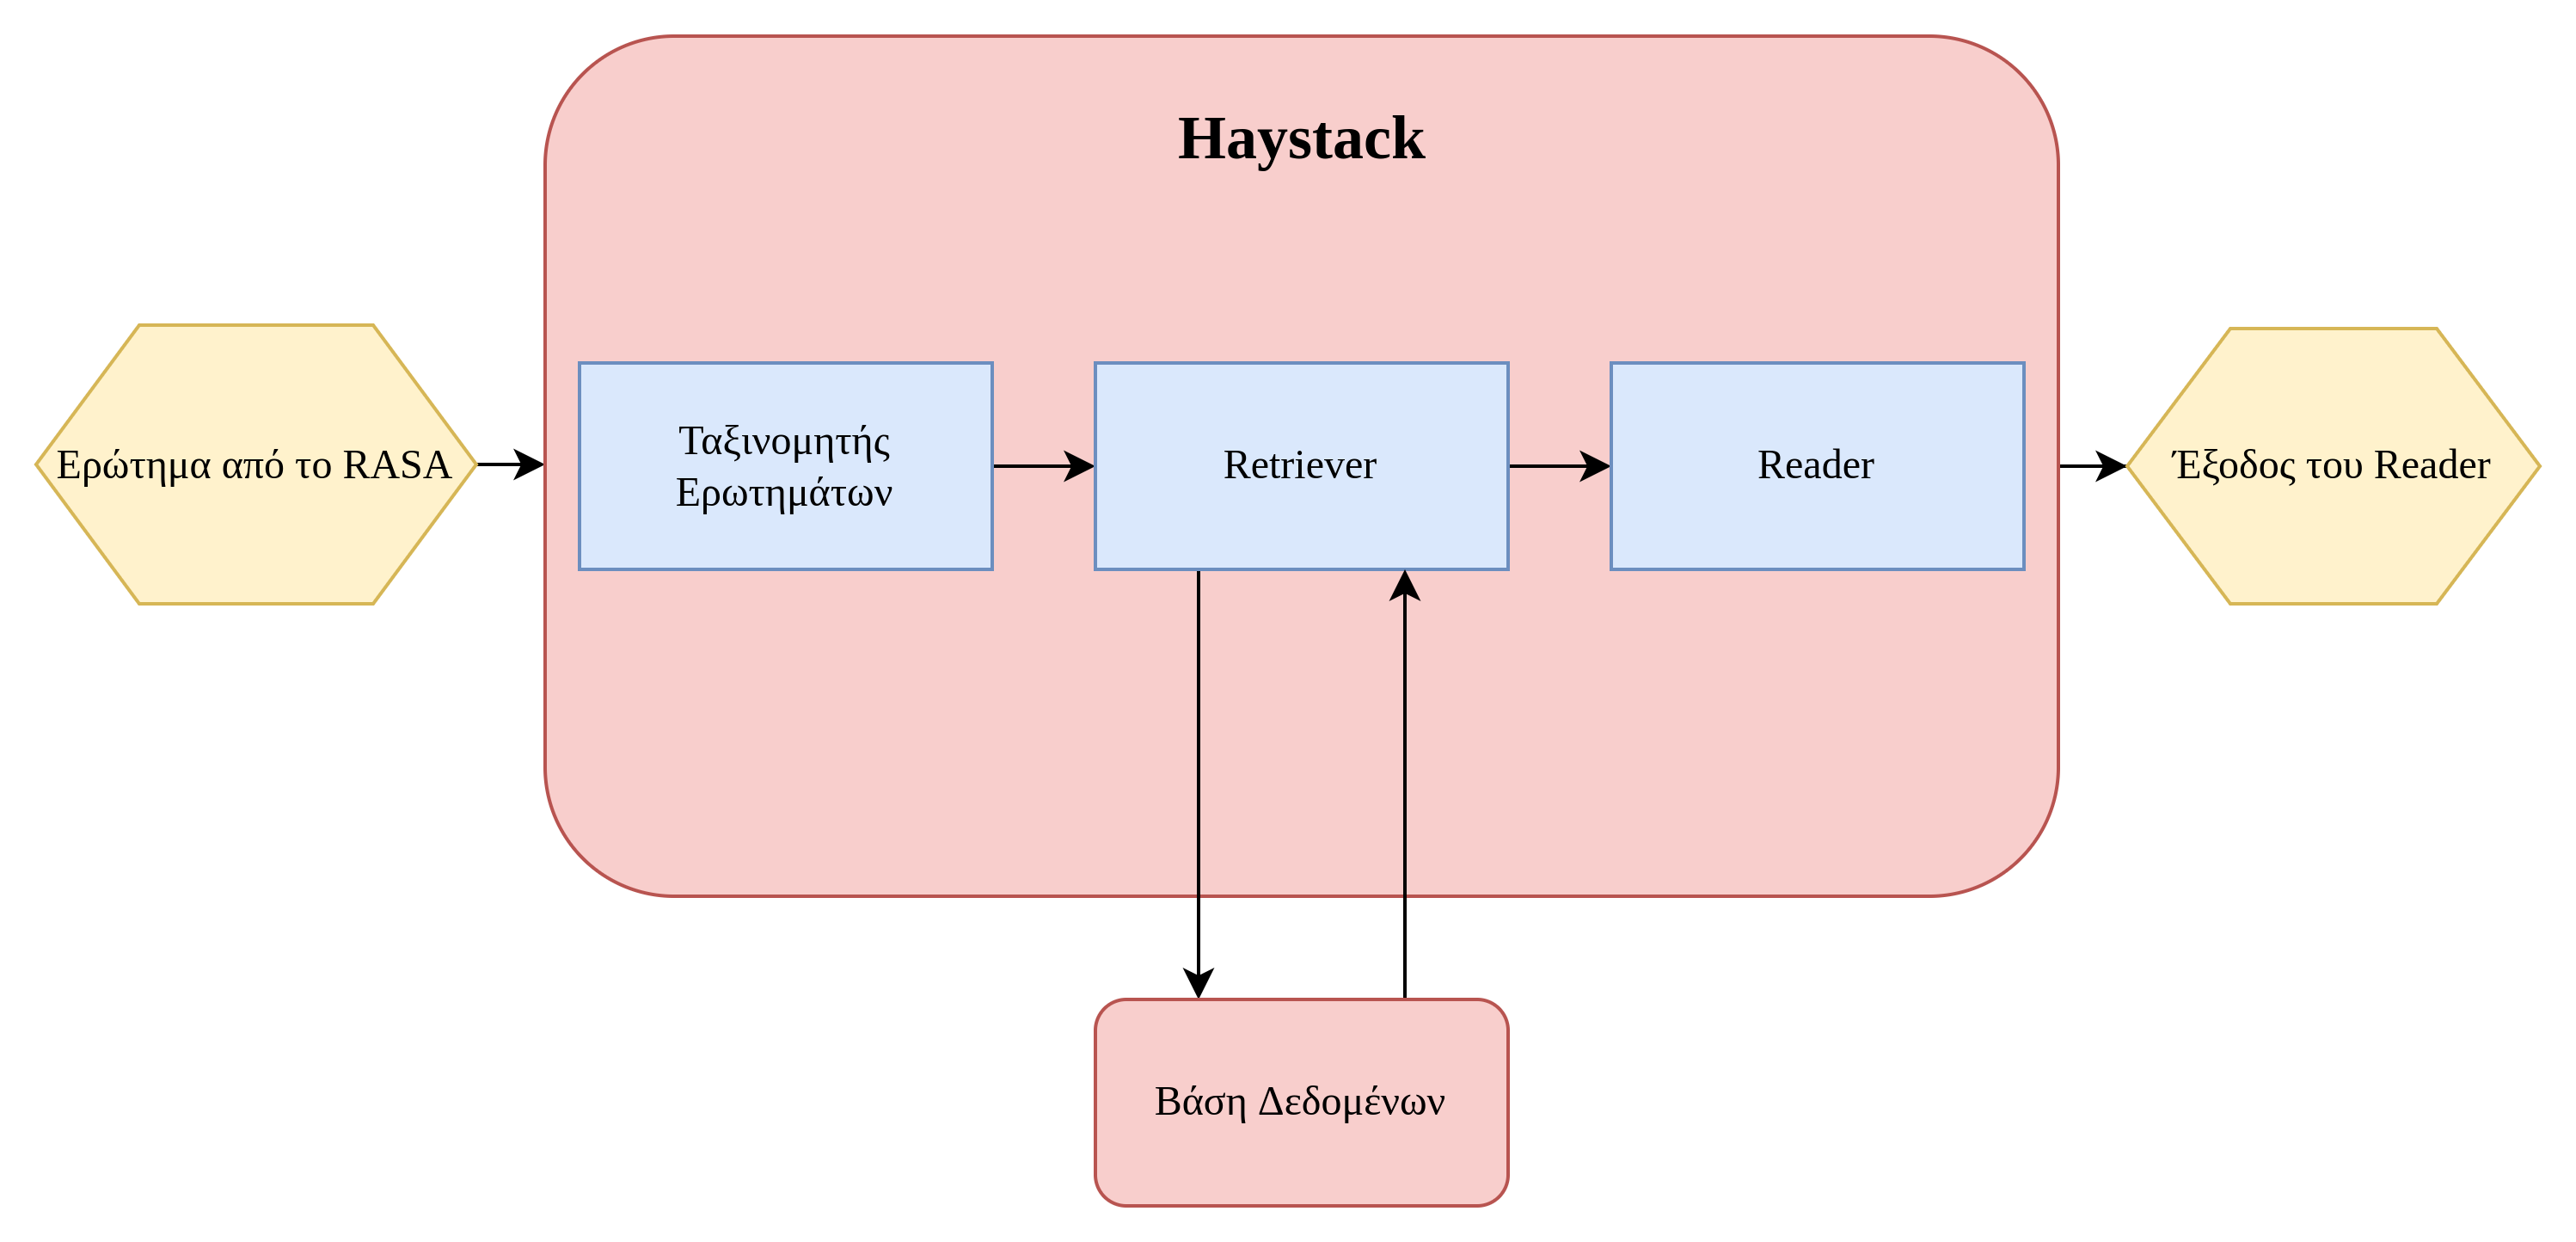
\includegraphics[width=1\textwidth]{images/chapter4/haystack.png}
  \caption{Haystack Pipeline}
  \label{fig:haystack-pipeline}
\end{figure}
\noindent